\documentclass[portrait,a4paper]{article}


\usepackage[utf8x]{inputenc}
\usepackage[T1]{fontenc}


\usepackage{mathtools}
\usepackage{amssymb,amsfonts,amsmath}
\usepackage[e]{esvect}

\usepackage{algorithmic}
\usepackage{algorithm}
\newcommand{\algorithmlabel}[2]{{
    \renewcommand{\algorithmicensure}{\textbf{#1}:}
    \ENSURE{#2~}
}}

\usepackage{graphicx}
\usepackage[svgnames]{xcolor}

\usepackage{geometry}
\geometry{a4paper}

% multirow and multicol
\usepackage{multirow}
\usepackage{multicol}
\columnsep24pt
\columnseprule0.1pt

% enumerate
\renewcommand\theenumi{\arabic{enumi}}
\renewcommand\labelenumi{\theenumi.}
\renewcommand\theenumii{\roman{enumii}}
\renewcommand\labelenumii{\theenumii)}

\usepackage{listings}
\lstset{
    floatplacement={tbp},
    basicstyle=\ttfamily\mdseries,
    identifierstyle=,
    stringstyle=\color{gray},
    numbers=left,
    numbersep=5pt,
    inputencoding=utf8x,
    xleftmargin=8pt,
    xrightmargin=8pt,
    keywordstyle=[1]\bfseries,
    keywordstyle=[2]\bfseries,
    keywordstyle=[3]\bfseries,
    keywordstyle=[4]\bfseries,
    numberstyle=\tiny,
    stepnumber=1,
    breaklines=true,
    frame=lines,
    showstringspaces=false,
    tabsize=2,
    commentstyle=\color{gray},
    captionpos=b,
    float=float,
    language={Java}
}
\newcommand{\code}[1]{\lstinline{#1}}

% hyperref
\usepackage[colorlinks=true,pdfborder={0 0 0},citecolor=DarkGreen,linkcolor=DarkBlue,urlcolor=DarkBlue]{hyperref}

% depth of section numbering
\setcounter{secnumdepth}{4}

% redefine the \paragraph command:
\makeatletter
\renewcommand\paragraph{\@startsection{paragraph}{4}{0mm}%
    {-\baselineskip}%
    {0.5\baselineskip}%
    {\normalfont\bfseries}%
}%
\makeatother

% new chapter command
\newcommand{\newchapter}{\clearpage\pagebreak}

% theorems
\usepackage{amsthm}
\newtheorem{lemma}{Lemma}[section]
\newtheorem{theorem}{Theorem}[section]
\newtheorem{corollary}{Corollary}[section]
\newtheorem{definition}{Definition}[section]
\newtheorem{remark}{Remark}[section]
\newtheorem{observation}{Observation}[section]
\newtheorem{assumption}{Assumption}[section]
\newtheorem{proposition}{Proposition}[section]

% autoref names
\newcommand{\specialref}[2]{\hyperref[#1]{#2~\ref*{#1}}}
\def\lstlistingautorefname{Listing}
\def\subsubsectionautorefname{Section}
\def\subsectionautorefname{Section}
\def\figureautorefname{Figure}

% parindent
\parindent0px
\parskip3pt

% redefine greek letters
\renewcommand{\phi}{\varphi}
\renewcommand{\epsilon}{\varepsilon}

% shortcuts in math mode
% \newcommand{\bs}{\boldsymbol}
\newcommand{\mc}{\mathcal}
\newcommand{\ds}{\displaystyle}
\DeclarePairedDelimiter\absimpl{\lvert}{\rvert}
\DeclarePairedDelimiter\normimpl{\lVert}{\rVert}
\newcommand{\abs}[1]{\absimpl*{#1}}
\newcommand{\norm}[1]{\normimpl*{#1}}
\newcommand{\argmax}{\operatorname*{arg\,max}}
\newcommand{\argmin}{\operatorname*{arg\,min}}

% number sets
\newcommand{\R}{\mathbb{R}}
\newcommand{\Z}{\mathbb{Z}}
\newcommand{\N}{\mathbb{N}}
\newcommand{\Q}{\mathbb{Q}}
\newcommand{\C}{\mathbb{C}}
\newcommand{\F}{\mathbb{F}}
\newcommand{\LL}{\mathcal{L}}
\newcommand{\powerset}{\mathcal P}

% probabilities
\newcommand{\Prob}[1]{\operatorname{Pr}\left[#1\right]}
\newcommand{\Ex}[1]{\mathbb{E}\left[#1\right]}

% misc
\newcommand{\bigO}[1]{\mc O\left(#1\right)} % big-o notation

\newcommand{\nop}[1]{} % temporarily remove from output




% todo
\usepackage{framed}
\newenvironment{todo}
{\color{DarkRed} \begin{leftbar}}
{\end{leftbar}}
\newcommand{\inlinetodo}[1]{{\textcolor{DarkRed}{ [\textbf{TODO}: #1]}}}
\newcommand{\mat}[1]{\bs{#1}}
\newcommand{\ma}{\mat{A}}
\newcommand{\mb}{\mat{B}}
\newcommand{\mx}{\mat{X}}
\newcommand{\mv}{\mat{V}}
\newcommand{\muu}{\mat{U}}
\newcommand{\md}{\mat{D}}
\newcommand{\ms}{\mat{S}}
\newcommand{\mz}{\mat{Z}}

\newcommand{\vx}{\mat{x}}
\newcommand{\va}{\mat{a}}
\newcommand{\vb}{\mat{b}}
\newcommand{\vu}{\mat{u}}
\newcommand{\vz}{\mat{z}}

\newcommand{\rd}{\R^D}
\newcommand{\rr}[2]{\R^{#1 \times #2}}

% \newcommand*{\titleSW}{\begingroup% Story of Writing
% \raggedleft
% \vspace*{\baselineskip}
% {\Huge\textbf{Computer Graphics}}\\[\baselineskip]
% {\large\textbf{ Exercise 1}}\\[\baselineskip]
% {\small Pascal Spörri (pascal@spoerri.io)}\

\usepackage{placeins}

\newcommand*{\titleSW}[3]{\begingroup% Story of Writing
\raggedleft
\vspace*{\baselineskip}
{\Huge\textbf{#1}}\\[0.7\baselineskip]
{\large\textbf{#2}}\\[0.5\baselineskip]
{\small #3}\par
\endgroup}

\begin{document}

 \author{Pascal Spörri\\pascal@spoerri.io}
 \title{HowTo Write Fast Numerical Code\\ Exercise 1}
 \date{\today}
\maketitle

\section{Cost Analysis}
We consider the matlab function given in the exercise sheet (listing \ref{listing:matlab}) provided on the course homepage:
\lstset{language=matlab}
\begin{lstlisting}[caption=Matlab code given in the exercise,label=listing:matlab]
function z = func (x1, x2, y)
    m = length(x1);
    n = length(y);
    if m == 1
        z = x1(1)+sum(y); 
    return    
    k = m/2;
    t = func(x1(1:k), x2(1:k), y)*func(x1(k+1:m), x2(k+1:m), y);
    x3 = x1+x2; 
    y1 = pi*y;
    z = t*func(x3(1:k), x3(k+1:m), y1);
end
\end{lstlisting}
\subsection{Floating Point Additions}
We observe that there are in total $A_1=n$ floating point additions for the case $length(x1)=m=1$ and 
\begin{align}
    A_m &= 3\cdot A_{m/2}+m
\end{align}
floating point additions per recursion step. Using the formula provided in the course we are able to solve the recursion by first substituting $m$ with $2^k$,
\begin{align}
    F_k = 3\cdot F_{k-1} + 2^k.
\end{align}
Then solving the recursion:
\begin{align}
    F_k = 3^k n + \sum_{i=0}^{k-1} 3^i \cdot 2^{k-i} = 3^k n - 2(2^k-3^k).
\end{align}
Doing a back substitution gives us a total amount of floating point additions:
\begin{align}
    A_m = 3^{\log_2{m}}n + 2(m-3^{\log_2{m}}).\label{eq:faAM}
\end{align}

\subsection{Floating Point Multiplications}
We observe that there are in total $M_1=0$ floating point additions for the case $length(x1)=m=1$ and 
\begin{align}
    M_m &= 3\cdot M_{m/2}+n+2
\end{align}
floating point multiplications per recursion step. Using the formula provided in the course we are able to solve the recursion:
\begin{align}
    G_0 &= 0,\\
    G_k &= 3\cdot G_{k-1} + n + 2&\text{Substitution of $m$ with $2^k$}\nonumber\\
        &= 3^k\cdot 0 + \sum_{i=0}^{k-1} 3^i\cdot (2+n)\nonumber\\
        &= \sum_{i=0}^{k-1} 3^i\cdot (2+n) = {1\over 2}\left(3^k-1\right)(n+2).\label{eq:fpGK}
\end{align}
By substituting back we get the total amount of floating point operations:
\begin{align}
    M_m &= {1\over 2}\left(3^{\log_2{k}}-1\right)(n+2).
\end{align}

\subsection{Total Floating Point Operations}
Adding the equations \eqref{eq:faAM} and \eqref{eq:fpGK} together we get the total amount of floating point operations in listing \ref{listing:matlab}:
\begin{align}
    C_m &=A_m+M_m \nonumber\\
     &= 3^{\log_2{m}}n + 2(m-3^{\log_2{m}}) + {1\over 2}\left(3^{\log_2{k}}-1\right)(n+2).
\end{align}

\section{Machine Information}

The computer is running a Mac OSX version 10.8.2 using a Intel Core i7-3720QM CPU using a frequency of 2.60 GHz per core. There are 4 cores (8 threads) available (Datasheet\footnote{\url{http://ark.intel.com/products/64891}}). 

Using an Intel Sandy Bridge architecture slideset\footnote{\url{https://www.cesga.es/gl/paginas/descargaDocumento/id/135}} and the architecture slides\footnote{\url{http://www.inf.ethz.ch/personal/markusp/teaching/263-2300-ETH-spring13/slides/arch.pdf}} we are able to compute the available floating point operations:
\begin{align}
    \text{Floating Point additions/cycle:}\quad &1\nonumber\\
    \text{Floating Point multiplications/cycle:}\quad &1\nonumber\\
    \text{GFlops/s:}\quad &\quad\ 2.6GHz \cdot 2 \text{Flops/cycle} \nonumber\\&= 5.6\ \text{GFlops/s per Core}\nonumber
\end{align}

\section{Matrix Multiplication}
In order to get accurate timings on OSX we installed and activated the DisableTurboBoost kernel module\footnote{\url{https://github.com/nanoant/DisableTurboBoost.kext}} on the computer. The \lstinline{sysctl} now shows:
\begin{lstlisting}[caption=Bash output of the sysctl command]
# sysctl -a hw | grep cpufrequency
hw.cpufrequency: 2600000000
hw.cpufrequency_min: 2600000000
hw.cpufrequency_max: 2600000000
hw.cpufrequency = 2600000000
\end{lstlisting}


The code shows $n\cdot m\cdot k$ floating point adds and $n\cdot m\cdot k$ floating point multiplications. \textbf{Total Floating Point operations: $\mathbf{2nmk}$}.

In order to get consistent timings we had to set the frequency define in \lstinline{mmm.c} to \lstinline{2.6e9}. Resulting in the following output:
\begin{lstlisting}[caption=Execution of the \lstinline{mmm.c} code compiled with GCC 4.7.2 and the flags \lstinline{-O3 -m64 -fno-tree-vectorize}.]
m=1000 k=1000 n=1000
RDTSC instruction:
 18399246918.000000 cycles measured => 7.076633 seconds, assuming frequency is 2600.000000 MHz. (change in source file if different)

C clock() function:
 7117748.000000 cycles measured. On some systems, this number seems to be actually computed from a timer in seconds then transformed into clock ticks using the variable CLOCKS_PER_SEC. Unfortunately, it appears that CLOCKS_PER_SEC is sometimes set improperly. (According to this variable, your computer should be running at 1.000000 MHz). In any case, dividing by this value should give a correct timing: 7.117748 seconds.

C gettimeofday() function:
 7.117292 seconds measured
\end{lstlisting}
\subsection{Plots}
\begin{figure}[H]
\centering
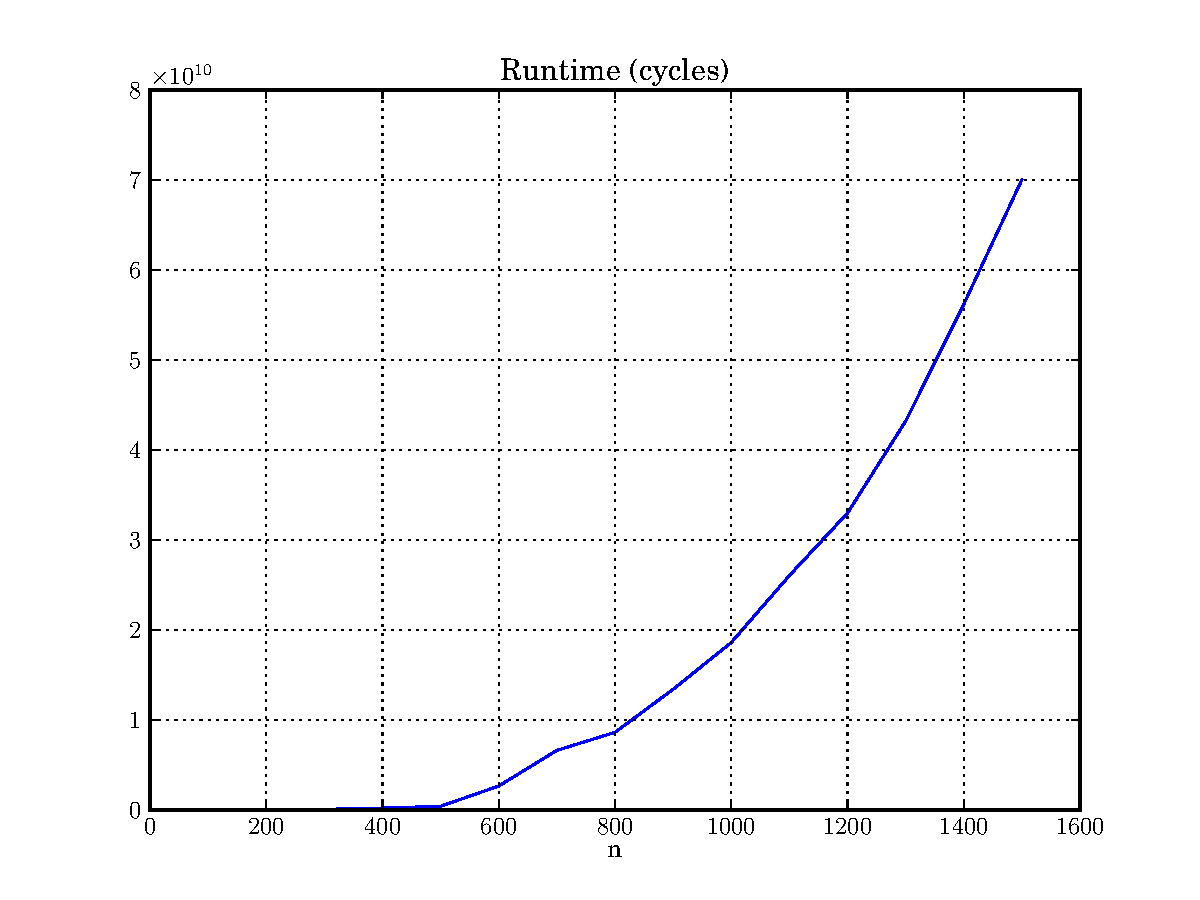
\includegraphics[width=0.7\textwidth]{mmm/Runtimecycles.pdf}
\caption{Runtime of \lstinline{mmm.c} in cycles. Compiler: GCC 4.7.2, Flags: \lstinline{-O3 -m64 -fno-tree-vectorize}.}
\end{figure}

\begin{figure}[H]
\centering
\includegraphics[width=0.7\textwidth]{mmm/GFlops.pdf}
\caption{Achieved GFlop/s of \lstinline{mmm.c} in cycles. Compiler: GCC 4.7.2, Flags: \lstinline{-O3 -m64 -fno-tree-vectorize}.}
\end{figure}

\begin{figure}[H]
\centering
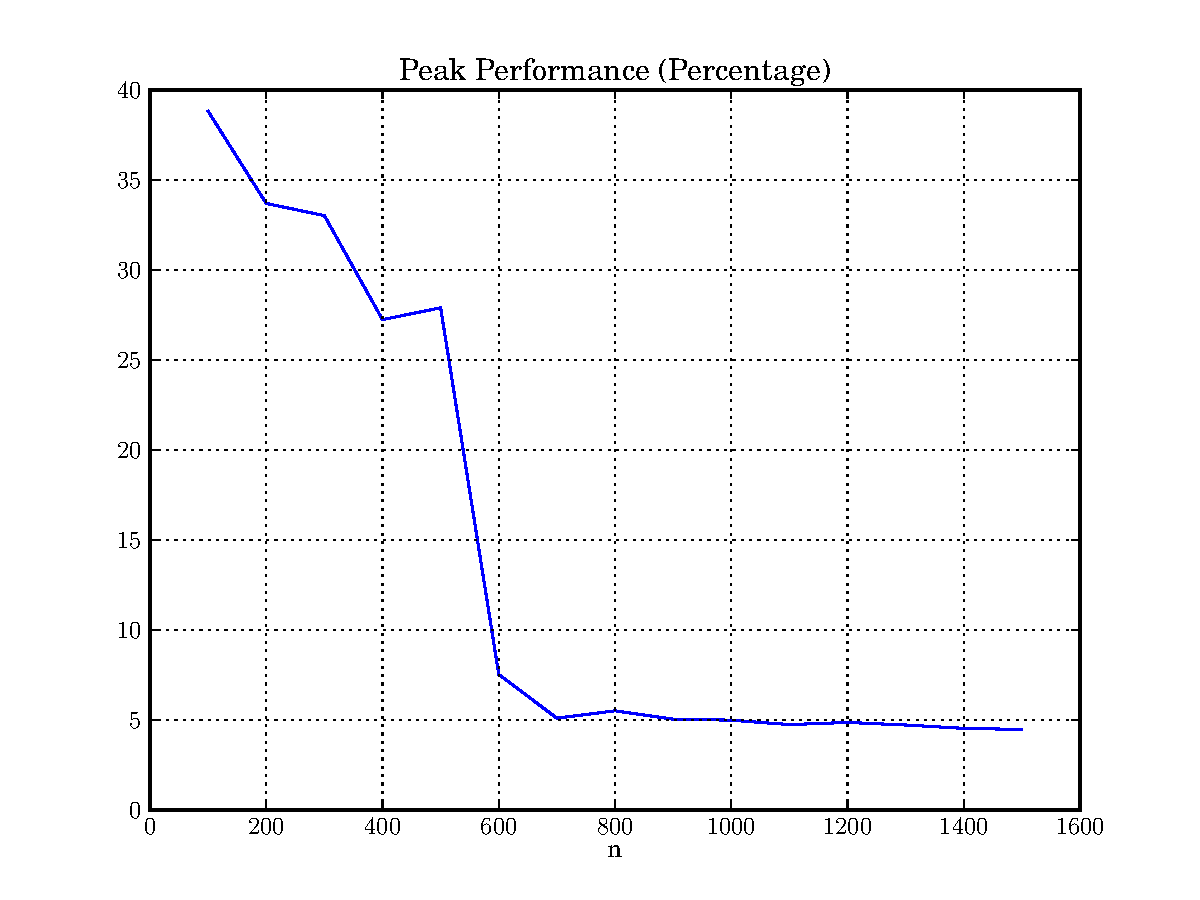
\includegraphics[width=0.7\textwidth]{mmm/PeakPerformancePercentage.pdf}
\caption{Achieved peak performance (percentage) of \lstinline{mmm.c} in cycles. Compiler: GCC 4.7.2, Flags: \lstinline{-O3 -m64 -fno-tree-vectorize}.}
\end{figure}
We observe that we don't manage to use the utilise all the available floating point units. 

\section{Daxpy}
The implementation of the ''daxpy'' function was straightforward. We copied the \lstinline{mmm.c} code and replaced the matrix multiplication with the vector addition. 

\subsection{Plots}
\begin{figure}[H]
\centering
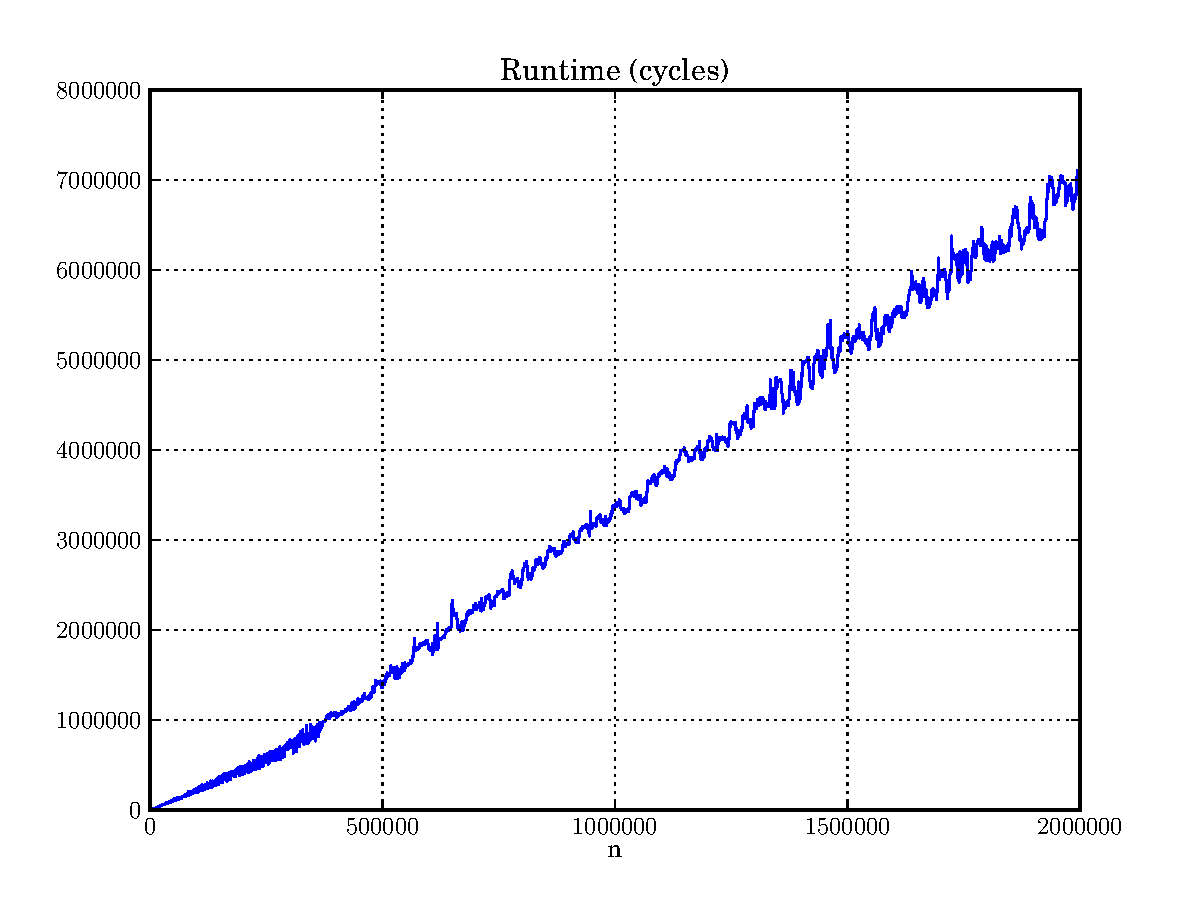
\includegraphics[width=0.7\textwidth]{daxpy/Runtimecycles.pdf}
\caption{Runtime of \lstinline{daxpy.c} in cycles. Compiler: GCC 4.7.2, Flags: \lstinline{-O3 -m64 -fno-tree-vectorize}.}
\end{figure}

\begin{figure}[H]
\centering
\includegraphics[width=0.7\textwidth]{daxpy/GFlops.pdf}
\caption{Achieved GFlop/s of \lstinline{daxpy.c} in cycles. Compiler: GCC 4.7.2, Flags: \lstinline{-O3 -m64 -fno-tree-vectorize}.}
\end{figure}

\begin{figure}[H]
\centering
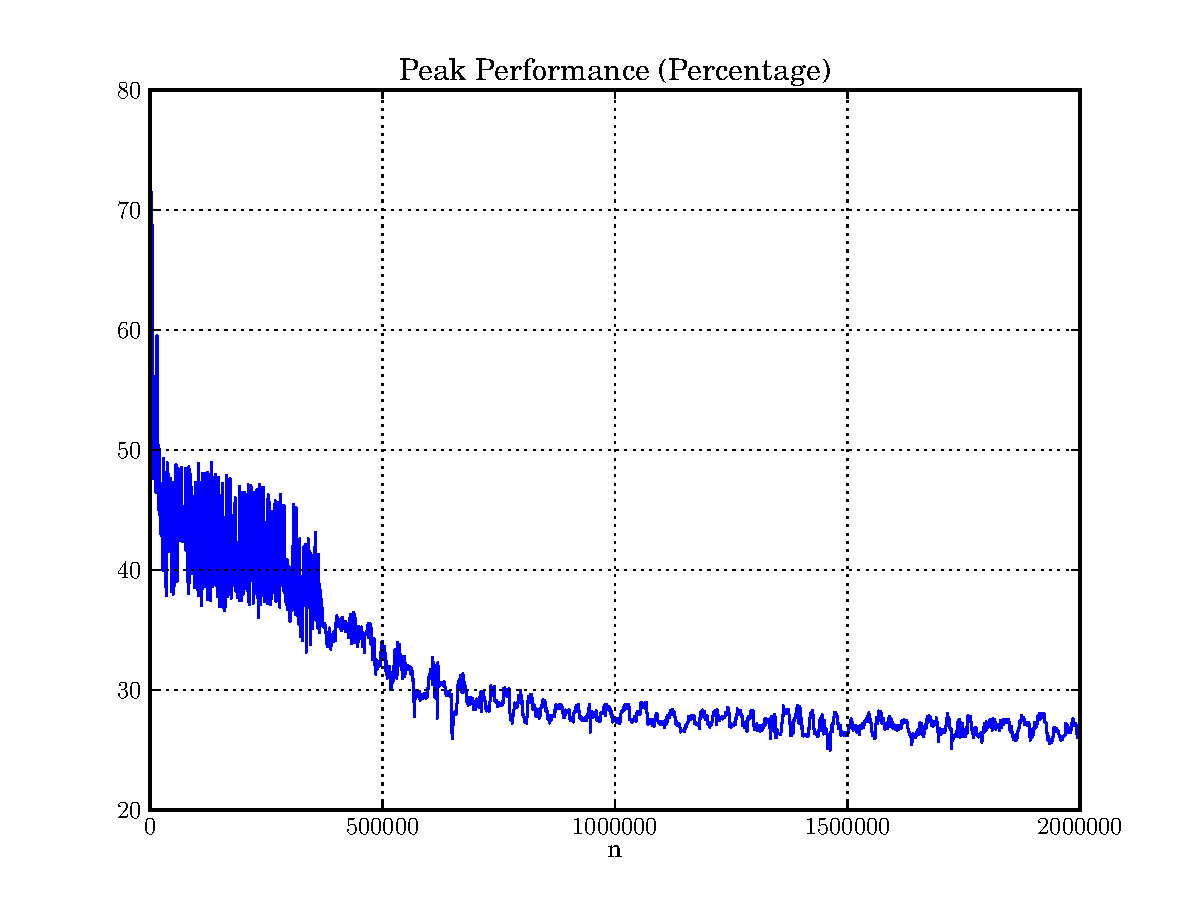
\includegraphics[width=0.7\textwidth]{daxpy/PeakPerformancePercentage.pdf}
\caption{Achieved peak performance (percentage) of \lstinline{daxpy.c} in cycles. Compiler: GCC 4.7.2, Flags: \lstinline{-O3 -m64 -fno-tree-vectorize}.}
\end{figure}

We notice that we were able to utilize 72\% of the available floating point peak performance using a vector length of $n=1000$.

\section{Bounds}

\end{document}
